\section{Theoretical Background} \label{sec:theory}
The purpose of this chapter is to go through the preliminary wind turbine (WT) theory. (Subject to change!)

\subsection{Aerodynamics and airfoil theory} \label{sec:theory_aero}
The sun delivers energy to the earth by heating up the surface and subsequently the air of the earth. Winds occur as a result of the pressure differences that occur due to the expansion and contraction of the air. 

WTs work because they are able to convert the wind's energy into a torque in the generator which then generates electrical energy. When the wind blows over the blades of a WT it delivers some of its energy to the blade, yielding both a thrust force and torque to the blade.

In the simplest 1D momentum theory case the delivery of energy just results in a lowing of the wind speed following the rotor area. Due to mass preservation an expansion would subsequently occur as depicted in \cref{fig:betz}.
\begin{figure}[h]
	\centering
	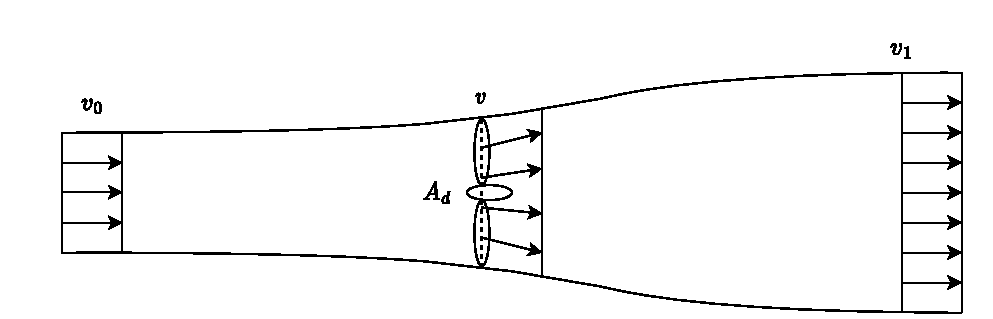
\includegraphics[width=0.8\linewidth]{Graphics/FlowThroughRotor.pdf}
	\caption{Illustration of how the wind in a control volume (CV) changes volume due to its reduction of speed}
	\label{fig:betz}
\end{figure}
The power of the \textit{free} wind $ v_0 $ can be expressed from the wind mass flow $ \dot{m} $ through a control volume:
\begin{equation} \label{eq:power}
	P = \dfrac{1}{2} \dot{m} v_0^2
\end{equation}
The flow of mass can be expressed from the air density $ \rho $, the cross sectional area $ A_d $ of the CV  at the rotor and the free wind speed $ v_0 $ as such:
\begin{equation}\label{eq:mass_deriv}
	\dot{m} = \rho A_d v_0
\end{equation}
Combining \cref{eq:power} and \cref{eq:mass_deriv} yields:
\begin{equation}\label{eq:power2}
	P_{air} = \dfrac{1}{2} \rho A_d v_0^3
\end{equation}
A \textit{power coefficient} $ C_p $ represents the percentage of the available power that is extracted from the wind:
\begin{equation}\label{eq:power_w_Cp}
	P_{T} = \dfrac{1}{2} \rho A_d v_0^3 C_p
\end{equation}
$ C_p $ is dependent on the rotor blade pitch $ \theta $ and the tip speed ratio (TSR) $ \lambda $. In the partial load region the goal is to reach a maximum $ C_p $ by adjusting $ \theta $ and  $ \lambda $ to their optimal values:
\begin{equation}\label{eq:cp_optimal}
	C_p^\star = C_p(\theta^\star, \lambda^\star)
\end{equation}
The TSR is the ratio between the speed of the tip of the WT blade $ (\Omega R) $ where $ R $ is the distance from the center of the rotor and the blade tip and the incoming free wind $v_0$:
\begin{equation}\label{eq:tipspeedratio}
	\lambda = \dfrac{\Omega R}{v_0}
\end{equation}

The achievable size of $ C_p^\star $ is a matter of the WT design. The \textit{Betz limit} is the highest, optimal $ C_p $ that can be theoretically achieved and can be calculated to be:
\begin{equation}\label{eq:betzlimit}
	C_{pbetz} = 0.5962
\end{equation}
%Most often $ C_p $ is also the measure of efficiency for a WT, but a more intuitive efficiency is  calculate measure efficiency from the Betz limit extractable power:
%\begin{equation}\label{eq:efficiency}
%	\eta = \dfrac{C_p}{C_{pbetz}}
%\end{equation}

%When the air travels over the WT blade the air travels slower on one side than the other as illustrated in \cref{fig:airfoil}. Due to mass conservation the air which moves slower on the underside of the blade expands, creating a higher pressure. Likewise the air moving faster on the upper upper side contracts creating in a lower pressure. Resultingly the blade moves upwards.
%\begin{figure}[h]
%	\centering
%	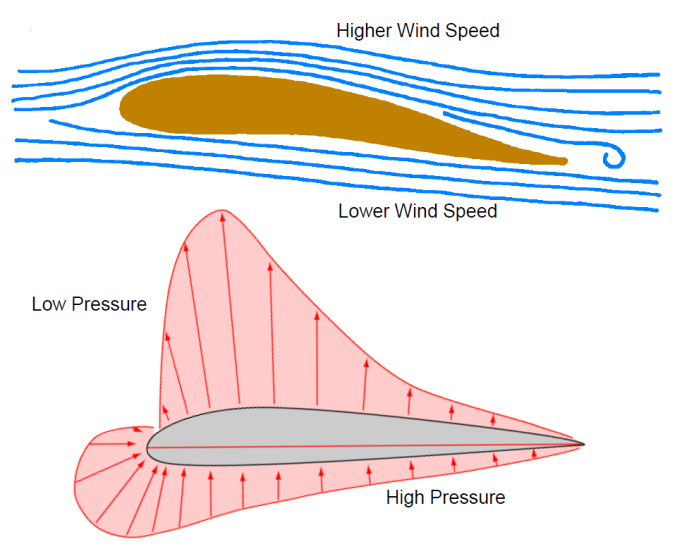
\includegraphics[width=0.5\linewidth]{Graphics/AirfoilAirflow.png}
%	\caption{Illustration of the wind speed difference between the two sides of a WT blade along with an illustration of the induced pressure difference. The result is a lifting force one the blade.}
%	\label{fig:airfoil}
%\end{figure}

Blade element momentum theory is often used to model the forces acting along WT blades. Blade element theory involves breaking a blade into small sections and determining the forces acting on each small section. In \cref{fig:blade_vel_triangle} a cross section of a WT blade can be seen. In this figure, as it is also illustrated at the rotor blade in \cref{fig:betz}, the wind velocity that hits the rotor blades is lowered indicated by the \textit{axial induction factor} $ a $. What is not observed in \cref{fig:betz} is that some of the energy of the wind also goes into driving an airstream around the back of the rotors in the opposite direction of the blade rotation, indicated by the \textit{tangential induction factor} $ a' $. This is known as \textit{swirl losses}.
\begin{figure*}[h]
	\centering
	\subfloat[Blade cross section]{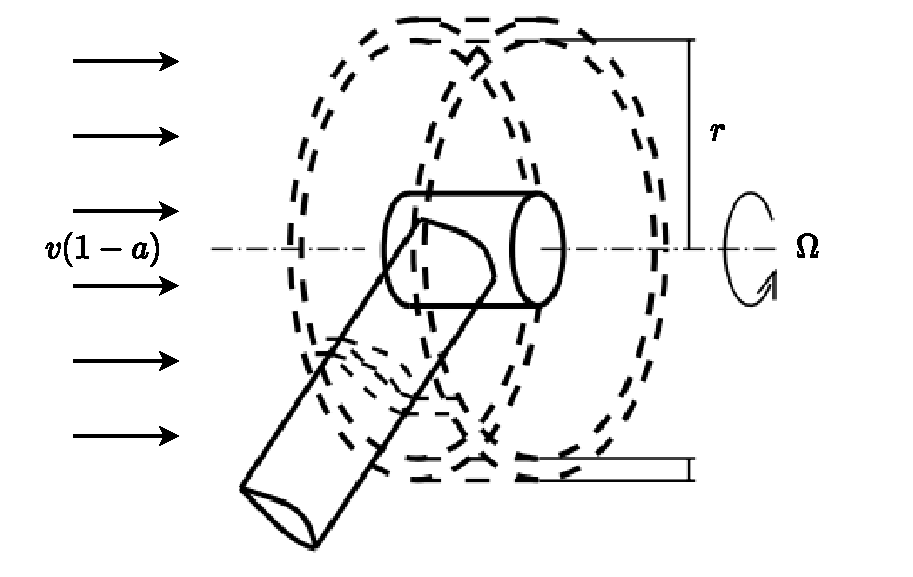
\includegraphics[width=.44\textwidth]{Graphics/RotorBladeElement.pdf}%
		\label{fig:blade_vel_triangles}}
	\hfil
	\subfloat[Velocity triangle]{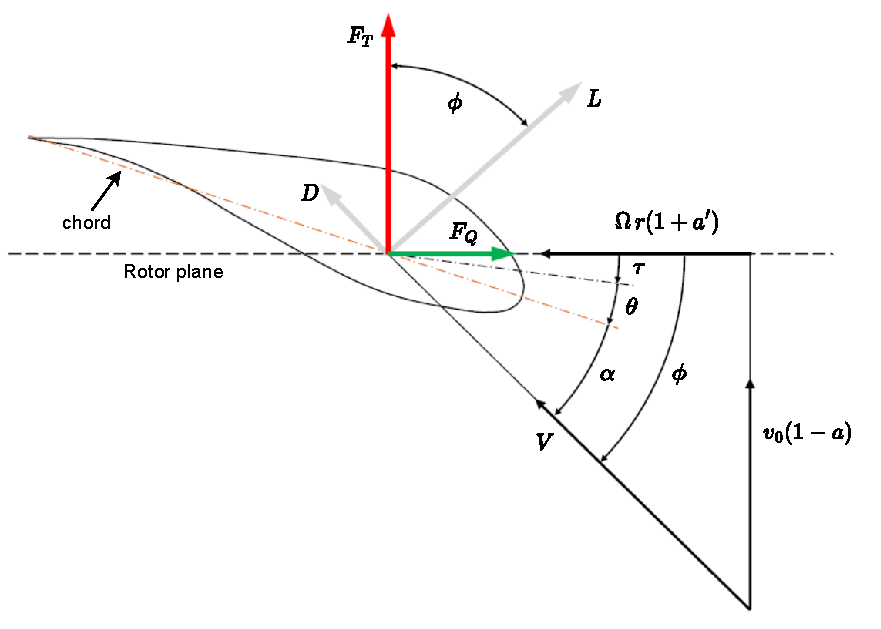
\includegraphics[width=.55\textwidth]{Graphics/BladeVelocityTriangle.pdf}%
		\label{fig:blade_vel_triangle}}
	\caption{Illustrations of a blade cross section and a velocity triangle on a blade section; \textbf{(a)} the blade cross section is made at some distance $ r $ from rotor center and rotates at a frequency $ \Omega $; \textbf{(b)} the velocity triangle acting on a cross section of a WT blade}
	\label{fig:blade_triangles}
\end{figure*}
The resulting air speed is V with an \textit{inflow angle} $ \phi $. $ F_L $ and $ F_D $ are the lift and drag forces on the blade element respectively. They are calculated from \cref{eq:lift} and \cref{eq:drag}. They include the \textit{chord length} $ c $ which is the length from the leading to the trailing edge of the blade.
\begin{align}
	F_L &= \dfrac{1}{2}\,  \rho \, V^2 c \, C_L \label{eq:lift}\\
	F_D &= \dfrac{1}{2} \, \rho \, V^2 c \, C_D \label{eq:drag}
\end{align}
The lift and drag coefficients $ C_L $ and $ C_D $ are usually extracted from table lookups which are typically found from simulations such as Xfoil
\todo{Hvad bruger Vestas til at finde $ C_L $ og $ C_D $?}. 
In a typical scenario $ C_L $ and $ C_D $ are found from the angle of attack $ \alpha $. The thrust and torque vectors $ F_T $ and $ F_Q $ are then calculated from the Pythagorean theorem as in \cref{eq:thrust} and \cref{eq:torque}
%\lipsum[11]\unsure{Is this correct?}\unsure{I'm unsure about also!}
\begin{align}\
	F_T &= L \, cos(\phi) + D \, sin(\phi) \label{eq:thrust} \\
	F_Q &= L \, sin(\phi) - D \, cos(\phi) \label{eq:torque}
\end{align}
The total thrust and torque of a blade can then be calculated by integrating the above over the length of the rotor blade.


\subsection{Wind turbine controller} \label{sec:theory_ctrl}